\renewcommand{\inputfile}{\version\ - edited 2007-03-11 symODEs}
% section: Symmetries of dynamical systems
% $Author$ $Date$

\subsection{Definition of symmetry}

We consider a system of \ode's of the form
\beq
	\dot{x} = \vf(x,\lambda)
	\label{eq:difeq}
\eeq
where $\vf: \Rls{n}\times\Rls{r}$ a $C^\infty$ mapping. When
not important we will suppress the $r$-dimensional vector of parameters
$\lambda$ in the notation.

As is well known any compact Lie group acting on $\Rls{n}$ can be identified
with a subgroup of $\On{n}$, \cf\ for example \refref{golubII}
for a sketch of the proof. Therefore, without loss of generality
we will concentrate on subgroups $\Gamma\subseteq\On{n}$ in the following.

\begin{definition}
\label{def:symmetry}
\index{symmetry}
We call a group element $\gamma\in\On{n}$ a symmetry of \refeq{eq:difeq} if for every solution
$x(t)$, $\gamma x(t)$ is also a solution.
\end{definition}

The question now arrises on how to check for symmetries of \refeq{eq:difeq} since
we generally do not have knowledge of the set of all solutions. Let $x(t)$ be a solution
of \ref{eq:difeq}. Then by \refDef{def:symmetry} $y(t)=\gamma x(t)$ is another solution 
and therefore satisfies \refneq{eq:difeq}:
\[
 \dot{y}(t)=\vf{y(t)}=\vf(\gamma x(t))\,.
\]
On the other hand
\[
 \dot{y}(t)=\gamma \dot{x} = \gamma \vf(x(t))\,,
\]
for any solution $x(t)$. Since solutions exist for any $x\in\Rls{n}$ we are led to the following 
condition for $\gamma$ to be a symmetry of \refeq{eq:difeq}:
\beq
	\vf(\gamma x) =\gamma \vf(x)
	\label{eq:equiv}
\eeq
for all $x\in\Rls{n}$. We say that $\vf$ \emph{commutes} with $\gamma$ or that $\vf$ is $\gamma$-\emph{equivariant}.
When $\vf$ commutes with all $\gamma\in\Gamma$ we say that $\vf$ is $\Gamma$-equivariant\index{equivariant}.
% When $f$ is $\gamma$-equivariant
% the \ode~ \ref{eq:difeq} remains invariant under the action of $\gamma$.

Clearly the finite time flow $\flow{t}{\gamma x_o}$ through $\gamma x_o$ 
satisfies the equivariance condition $\flow{t}{\gamma x_o}=\gamma \flow{t}{x_o}$ from 
the definition of symmetry and uniqueness of solutions.


\index{Lorenz equations!symmetry}For example, the vector field in Lorenz equations  \refneq{eq:lorenz} is equivariant under the group
$\Zn{2}\cong\Dn{1}$ acting on \Rls{3} by
\[
	\Rot{\pi}(x,y,z) = (-x,-y,z)\,.
\]
Notice that this transformation can be considered as either as rotation by $\pi$ around the $z$ axis (hence the
group \Zn{2}) or as a reflection about the origin in a plane perpendicular to the $z$-axis (hence the group \Dn{1}).

\index{Complex Lorenz equations!symmetry}As another example, the vector field in \CLe~ \refneq{eq:CLe} is equivariant under the group \SOn{2} acting on $\Rls{5}\cong \Clx{2}\times \Rls{}$
by
\beq
 \Rot{\theta} (x,y,z) = (e^{i\theta} x, e^{i\theta} y, z)\,,\ \ \  \theta\in[0,2\pi)\,.
 \label{eq:RotCLe}
\eeq

\index{Armbruster-Guckenheimer-Holmes flow!symmetry}Finally, the symmetry group of the \AGHe~\refneq{eq:AGH} is \On{2} acting by
\begin{eqnarray*}
  \Rot{\theta}(z_1,z_2) &=& (e^{i\theta} z_1, e^{i 2\theta} z_2)\,,\ \ \  \theta\in[0,2\pi)\,,\\
  \Refl(z_1,z_2) &=& (\conj{z}_1,\conj{z}_2)\,.
\end{eqnarray*}


\subsection{Phase space stratification}

In order to understand the implications of equivariance for the solutions
of \refeq{eq:difeq} we first have to closely examine the way a compact 
Lie group acts on \Rls{n}.

\index{group orbit} The \emph{group orbit} of $x\in\Rls{n}$ is the set
\beq
	\Gamma x = \{\gamma x: \gamma\in\Gamma\}\,.
\eeq

\index{isotropy subgroup}\index{stabilizer} Define the \emph{isotropy subgroup} or \emph{stabilizer} of $x\in\Rls{n}$ as
\beq
	\Sigma_x=\{\gamma\in\Gamma:\gamma x=x\}\,.
\eeq
Thus the isotropy subgroup describes the symmetries of a point $x$. The following usefull lemma
relates the isotropy subgroups of points on the same group orbit.

\begin{lemma}
\label{lm:stabGorbit}
Points on the same group orbit of $\Gamma$ have conjugate isotropy subgroups:
\beq
	\Sigma_{\gamma x}=\gamma \Sigma_x \gamma^{-1}\,.
\eeq
\end{lemma}
See \refref{golubII} for the proof.

\refLem{lm:stabGorbit} implies that we can characterize a group orbit by its \emph{type}, defined
as the conjugacy class of its isotropy subgroups.

\begin{proposition}
 Let $\Gamma$ be a compact Lie group acting on \Rls{n}. Then
 \begin{enumerate}
  \item If $\Gamma$ is finite then $|\Gamma|=|\Sigma_x||\Gamma x|$.
  \item If $\Gamma$ is continuous then $\dim \Gamma = \dim \Sigma_x+\dim \Gamma x$.
 \end{enumerate}
\end{proposition}
The proof can be found in \refref{golubII}. We note a usefull relation from the proof: $\dim\Gamma x =\dim(\Gamma/\Sigma_x)$, where the \emph{coset space} of a subgroup $\Sigma$  of $\Gamma$ is defined as $\Gamma/\Sigma=\{\gamma\Sigma|\gamma\in\Gamma\}$. Also recall that the (left) \emph{cosets} of $\Sigma$ in $\Gamma$ are the sets $\gamma\Sigma=\{\gamma\sigma|\sigma\in\Sigma\}$.

\index{stratum} 
Therefore, when $\Gamma$ is continuous each group orbit is a smooth compact manifold of dimension
$\dim \Gamma x=\dim \Gamma-\dim \Sigma_x$. The union of orbits of the same type is called a \emph{stratum}
and is itself a smooth manifold. Thus \Rls{n} is stratified by the action of $\Gamma$ into
a disjoint union of strata which are in an $1-1$ correspondance to the group orbit types. Notice that in general
the strata do not have the same dimension.



% The notion of equivariance is related to the symmetries of the \ode\ \refeq{eq:difeq}. We will also
% be interested on the symmetries of solutions.

\subsection{An example from laser theory}

Here we consider the $\SOn{2}$ equivariant \CLe~\refneq{eq:CLe} which as we mentioned
has been introduced in the study of baroclynic instability. We rewrite the system in
real variables $x=x_1+ i\, x_2\,,\ y=y_1+i\, x_2$ as
\beq
\begin{split}
	\dot{x}_1 &= -\sigma x_1 + \sigma y_1\cont
	\dot{x}_2 &= -\sigma x_2 + \sigma y_2\cont
	\dot{y}_1 &= (r_1-z) x_1 - r_2 x_2 -y_1-e y_2 \cont
	\dot{y}_2 &= r_2 x_1 + (r_1-z) x_2 + e y_1- y_2\cont
	\dot{z} &= -b z + x_1 y_1 + x_2 y_2\,.
	\label{eq:CLeR}
\end{split}
\eeq

The \stabmat\ is
  \beq
{\Mvar_{CLe}} =
  \left(\barr{ccccc}
    -\sigma    	& 0 		& \sigma & 0    &  0 \\
	0 	& -\sigma       & 0      & -\sigma   &  0 \\
	r_1-z  &     -r_2      & -1     & -e & -x_1 \\
	r_2     & r_1-z       	& e  	& -1       & -x_2 \\
	y_1     & y_2           & x_1    & x_2      & -b
    \earr\right)
\,.
  \ee{CLeStabMat} 

The origin is a fixed point of \refeq{eq:CLeR} for any value of the parameters. As shown in
\refref{FowlerCLE82} it is stable for $0<r_1<r_{1c}$ and unstable for $r_{1c}<r_1$, where
\beq
	r_{1c} = 1 + \frac{(e+r_2)(e-\sigma r_2}{(\sigma+1)^2}\,.
\eeq
At bifurcation a pair of eigenvalues crosses the imaginary axis with imaginary part:
\beq
	\omega_c = \frac{\sigma (e + r_2)}{\sigma+1}\,.
	\label{eq:omegaCLE}
\eeq

Thus we can expect that after a center manifold or Liapunov-Schmidt reduction one
can apply the equivariant Hopf bifurcation theorem\ES{state it in appropriate section,
refer to it.} with $\SOn{2}$ symmetry thus
concluding the existance of a relative equilibrium after bifurcation\ES{I'll do this
if I have time.}. In \refref{FowlerCLE82} the authors perform a direct bifurcation analysis and
show that, for $e+r_2\neq 0$, a Hopf cycle is created that also turns out to be an \SOn{2}-orbit, 
\ie a relative equilibrium. For $e+r_2=0$ the cycle degenerates to an \SOn{2}-orbit of equilibria $E_1$,
since $\omega_c =0$ and the conditions of equivariant Hopf theorem do not apply. 

The secondary bifurcation from the relative equilibrium is expected according to Krupa's theorem\ES{refer to it
when written up} to result in relative periodic orbits. In the non-generic case of an \SOn{2}-orbit of equilibria
it has been shown by Krupa that one gets bifurcation to periodic orbits. The secondary bifurcation has
been studied in \cite{NingHakenCLE90}\ES{The results are messy and hard to comment on.
They show existence of supercritical and subcritical bifurcations. Will continue this discussion
later}. 

Ning and Haken~\cite{NingHakenCLE90} have shown that certain semiclassical approximations
for single mode, detuned, ring lasers lead to equations isomorphic to \CLe. %with $x,y$ and $z$ 
%proportional to electric field, polarization and population inversion, respectively. 
The authors in \refref{NingHakenCLE90}
make the choice $e+r_2=0$ so that a detuned stationary solution exists.\ES{This assumption is
questionable unless it is forced by the physics of the problem, which I cannot follow very
well. It leads to non-generic bifurcation behaviour, while one would like a model of
a physical system to be robust under perturbations (of the model). Furthermore, the fact that the
Hopf cycle in the general case is an $\SOn{2}$-orbit has gone unnoticed. The relative equilibrium can
be interpreted as an equilibrium in a rotating frame and the measured electric field of the laser
would be the same in both cases.}

\subsubsection{The $e=r_2=0$ case}

When one takes $e=r_2=0$ we immediatelly observe the real subspace $x_2=y_2=0$ is flow invariant
and the usual \Le\ are recovered. From equivariance, any subspace $U_\theta$ on the $\SOn{2}$-orbit of the real
subspace is invariant as well, for example the imaginary subspace $x_1=y_1=0$. The
$U_\theta$'s are  parametrized by the angle of \SOn{2} rotations with 
the restriction $\theta\in[0,\pi)$. We demonstrate the situation for the standard \Le\ parameters 
in \reffig{fig:LorenzCoex}. A continuum of identical, disjoint Lorenz ``butterfly'' attractors exists.

%%%%%%%%%%%%%%%%%%%%%%%%%%%%%%%%%%%%%%%%%%%%%%%%%%%%%%%%%%%%%%%%%%
\begin{figure}[t]
\begin{center}
  (\textit{a})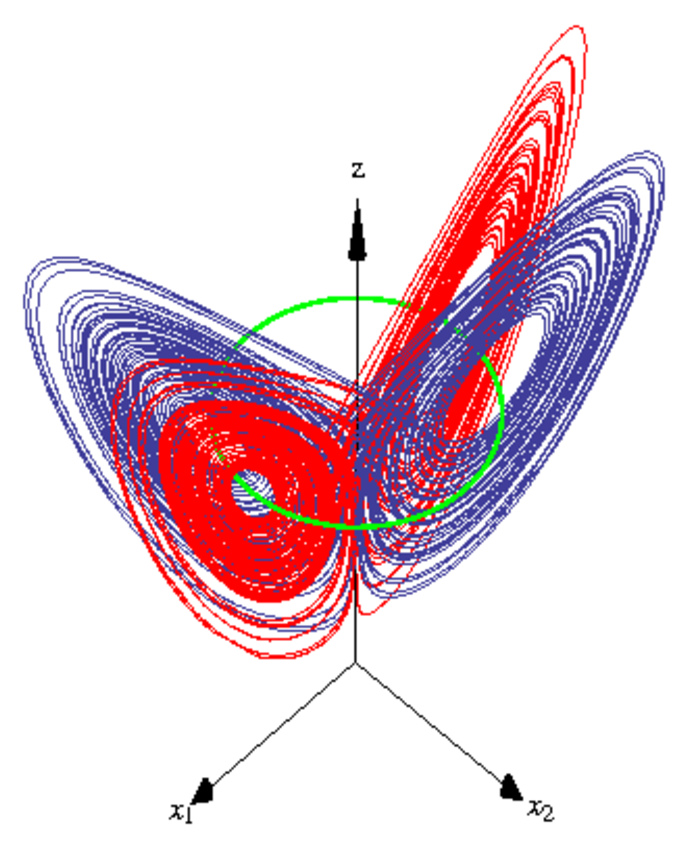
\includegraphics[width=0.35\textwidth]{../figs/LorenzCoexA.eps}
~~~~(\textit{b})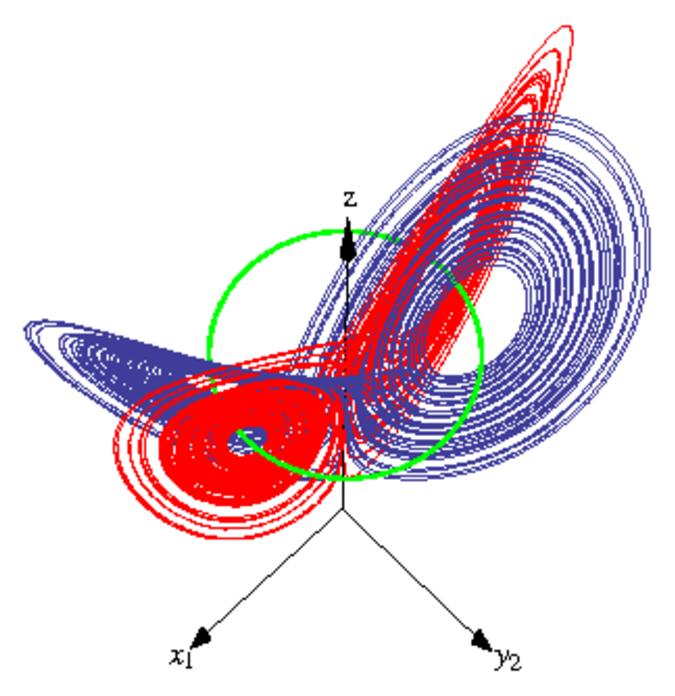
\includegraphics[width=0.35\textwidth]{../figs/LorenzCoexB.eps}
\end{center}
\caption[Complex Lorenz eq. coexisting attractors]{ Two different projections
of the \CLe dynamics for $r_1=28,\, b=8/3,\, \sigma=10,\, a=1$ and $e=r_2=0$. The dynamics in
the real subspace $U_0$ and in $U_{5\pi/6}$ is shown in red, blue respectively. The green circle
represents the \SOn{2}-orbit of equilibria $E_1$.
    }
\label{fig:LorenzCoex}
\end{figure}
%%%%%%%%%%%%%%%%%%%%%%%%%%%%%%%%%%%%%%%%%%%%%%%%%%%%%%%%%%%%%%%%


Yet, we have to notice that we cannot choose all initial conditions
in one of the flow invariant subspaces $U_\theta$. Indeed, if we use the real subspace
as reference we can choose coordinates $(x_1,y_1,z,\theta)$ for the subspace $U$ of \Rls{5} 
foliated by the $U_\theta$'s, which makes it clear that this is a 4-dimensional subspace.
Points that do not lie on $U$ can be thought of as ``mis-rotated'': we start with a point on
the real subspace and rotate by an angle $\theta$ on the $(x_1,x_2)$-plane and by an
angle $\phi\neq\theta$ on the $(y_1,y_2)$ plane. One then would like to know where the asymptotic dynamics
for those initial conditions not in $U$ end up. Since the only equilibria of the equations are the origin
and the group orbit of equilibria $E_1$, we get the hint that the asymptotic dynamics has to be governed
by the stable and unstable manifolds of the same equilibria that govern dynamics in $U$.
To see whether this is true we examine the dot product of the vector field with the direction of
rotations of the system
% \beq
%   (x_2\ -x_1\ y_2\ -y_1)
%     \left(\barr{c}
% 	 -\sigma x_1 + \sigma y_1 \\
% 	 -\sigma x_2 + \sigma y_2 \\
% 	 (r_1-z) x_1 - r_2 x_2 -y_1-e y_2 \\
% 	 r_2 x_1 + (r_1-z) x_2 + e y_1- y_2\\
% 	 -b z + x_1 y_1 + x_2 y_2\,.
%     \earr\right)
% \,.
% \eeq
\beq
	(\Lg.p).\vf(p) = \left(r_1-\sigma-z\right)\left(x_1 y_2 -x_2 y_1\right) -r_2\left(x_1 y_1+ x_2 y_2\right)- e\left(y_1^2+y_2^2\right)
	\label{eq:CLe0ip}
\eeq
where we have used $\Lg$, the Lie algebra generator of \SOn{2}, $p=(x_1,x_2,y_1,y_2)$ and $\vf(p)$ the vector field in \refeq{eq:CLeR}.
We observe that for $e=r_2=0$ only $x_1 y_2-x_2 y_1$ and $z$ appear. By taking the time derivative of $x_1 y_2-x_2 y_1$ and using \refeq{eq:CLeR} 
we can show that
\beq
	\frac{d}{dt}\left(x_1 y_2-x_2 y_1\right)= -(\sigma+1)\left(x_1 y_2-x_2 y_1\right)
\eeq
and, since $z$ is bounded, the inner product in \refeq{eq:CLe0ip} goes to zero as $t\rightarrow\infty$. Thus, asymptotically the vector
field along any trajectory becomes orthogonal to the direction of infinitesimal rotations and the dynamics approach one of the $U_\theta$'s.
This is demonstrated in \reffig{fig:CLe0trans}.

%%%%%%%%%%%%%%%%%%%%%%%%%%%%%%%%%%%%%%%%%%%%%%%%%%%%%%%%%%%%%%%%%%
\begin{figure}[t]
\begin{center}
  (\textit{a})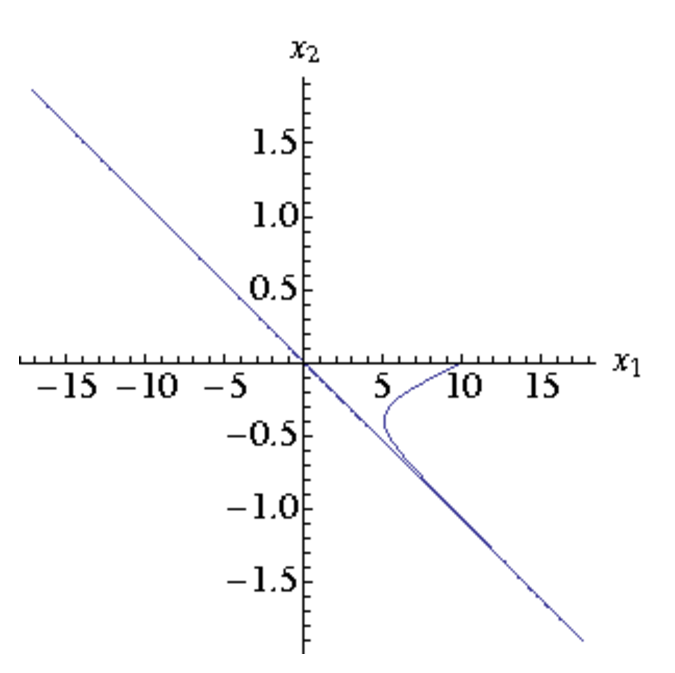
\includegraphics[width=0.35\textwidth]{../figs/CLe0transA.eps}
~~~~(\textit{b})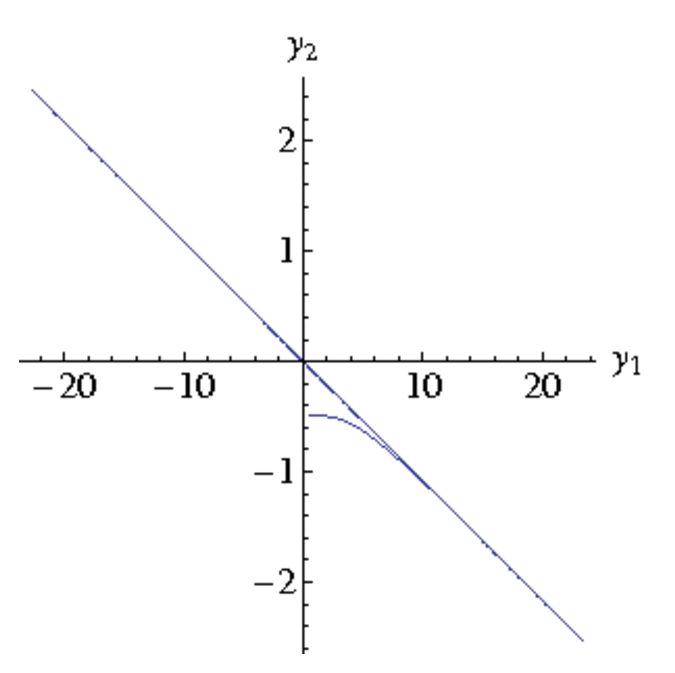
\includegraphics[width=0.35\textwidth]{../figs/CLe0transB.eps}
\end{center}
\caption[Transient trajectory in degenerate Complex Lorenz eq.]{ A trajectory
of the \CLe dynamics for $r_1=28,\, b=8/3,\, \sigma=10,\, a=1$ and $e=r_2=0$ with
initial conditions on the complement of $U$ in \Rls{5}. (a) Projection on the
complex $x$-plane, (b) Projection on the complex $y$-plane. The trajectory
approaches some $U_\theta$.
    }
\label{fig:LorenzCoex}
\end{figure}
%%%%%%%%%%%%%%%%%%%%%%%%%%%%%%%%%%%%%%%%%%%%%%%%%%%%%%%%%%%%%%%%